\documentclass[12pt,a4paper]{article}

% ─── Page Layout ───────────────────────────────────────────────────────────────
\usepackage[a4paper, margin=0.8in, headheight=14pt]{geometry}

% ─── Fonts (XeLaTeX) ───────────────────────────────────────────────────────────
\usepackage{fontspec}
\usepackage{unicode-math}
\setmainfont{TeX Gyre Pagella}
\setmonofont[Scale=0.88]{TeX Gyre Cursor}
\setmathfont{Latin Modern Math}

% ─── Packages ──────────────────────────────────────────────────────────────────
\usepackage{xcolor}
\usepackage{colortbl}
\usepackage{titlesec}
\usepackage{enumitem}
\usepackage{tabularx}
\usepackage{booktabs}
\usepackage{array}
\usepackage{amsmath}
\usepackage{tikz}
\usetikzlibrary{shapes.geometric, arrows.meta, positioning, calc, fit, decorations.pathreplacing}
\usepackage{tcolorbox}
\tcbuselibrary{skins, breakable}
\usepackage{hyperref}
\usepackage{fancyhdr}
\usepackage{graphicx}
\usepackage{microtype}
\hyphenpenalty=10000
\exhyphenpenalty=10000
\sloppy
\usepackage{caption}
\usepackage{setspace}
\usepackage{multirow}
\usepackage{tocloft}

% ─── Q&A helper ────────────────────────────────────────────────────────────────
\newcommand{\Q}[1]{\textbf{#1}\par\noindent\ignorespaces}

% ─── Colour Palette ────────────────────────────────────────────────────────────
\definecolor{myred}{RGB}{196,30,58}
\definecolor{mydark}{RGB}{30,30,50}
\definecolor{mygreen}{RGB}{14,120,80}
\definecolor{myteal}{RGB}{0,130,140}
\definecolor{myamber}{RGB}{180,100,0}
\definecolor{mypurple}{RGB}{100,30,160}
\definecolor{mygray}{RGB}{246,247,249}
\definecolor{mgframe}{RGB}{180,185,200}
\definecolor{watermark}{RGB}{145,150,170}
\definecolor{hdrred}{RGB}{250,232,235}
\definecolor{hdrgreen}{RGB}{220,244,233}
\definecolor{hdrteal}{RGB}{220,242,244}
\definecolor{hdramber}{RGB}{253,242,215}
\definecolor{hdrpurple}{RGB}{238,228,255}
\definecolor{hdrgray}{RGB}{238,240,245}
\definecolor{rowalt}{RGB}{250,251,253}

% ─── Section Formatting ────────────────────────────────────────────────────────
\titleformat{\section}
  {\large\bfseries\color{myred}}{\thesection.}{0.5em}{}
  [\vspace{1pt}{\color{myred}\rule{\linewidth}{0.8pt}}]
\titleformat{\subsection}
  {\normalsize\bfseries\color{myteal}}{\thesubsection}{0.5em}{}
\titlespacing*{\section}{0pt}{18pt}{7pt}
\titlespacing*{\subsection}{0pt}{11pt}{4pt}

% ─── Paragraph ─────────────────────────────────────────────────────────────────
\setlength{\parindent}{0pt}
\setlength{\parskip}{4pt}

% ─── TOC Styling ───────────────────────────────────────────────────────────────
\renewcommand{\cfttoctitlefont}{\large\bfseries\color{myred}}
\renewcommand{\cftaftertoctitle}{\par\noindent{\color{myred}\rule{\linewidth}{0.8pt}}}
\setlength{\cftbeforetoctitleskip}{0pt}
\setlength{\cftaftertoctitleskip}{6pt}
\renewcommand{\cftsecfont}{\normalsize\bfseries\color{mydark}}
\renewcommand{\cftsecpagefont}{\normalsize\bfseries\color{mydark}}
\renewcommand{\cftsecleader}{\cftdotfill{\cftdotsep}}
\setlength{\cftbeforesecskip}{7pt}
\renewcommand{\cftsubsecfont}{\small\color{mydark}}
\renewcommand{\cftsubsecpagefont}{\small\color{mydark}}
\setlength{\cftbeforesubsecskip}{3pt}
\setlength{\cftsubsecindent}{1.4em}

% ─── Table helpers ─────────────────────────────────────────────────────────────
\renewcommand{\arraystretch}{1.45}
\setlength{\tabcolsep}{6pt}
\arrayrulecolor{mydark}
\newcolumntype{B}[1]{>{\small\bfseries\raggedright\arraybackslash}m{#1}}
\newcolumntype{Y}{>{\small\raggedright\arraybackslash}X}
\renewcommand{\tabularxcolumn}[1]{m{#1}}

% ─── Header / Footer ───────────────────────────────────────────────────────────
\pagestyle{fancy}
\fancyhf{}
\fancyhead[L]{\small\color{myred}\textbf{OE-EC704B}\;\color{mydark}--- Optimization Technique}
\fancyhead[R]{\small\color{myteal}\textbf{Module 6 Notes}}
\fancyfoot[C]{\small\color{mydark}\thepage}
\fancyfoot[R]{\small\color{watermark}\textit{\copyright\ Biraj}}
\renewcommand{\headrulewidth}{0.5pt}
\renewcommand{\footrulewidth}{0.3pt}

% ─── Hyperref ──────────────────────────────────────────────────────────────────
\hypersetup{
  colorlinks=true, linkcolor=myteal, urlcolor=myteal,
  pdfauthor={Biraj Sarkar},
  pdftitle={OE-EC704B --- Module 6 Notes}
}

% ─── tcolorbox styles ──────────────────────────────────────────────────────────
\tcbset{
  tikzbox/.style={
    colback=mygray, colframe=mgframe, boxrule=0.6pt, arc=4pt,
    left=8pt, right=8pt, top=6pt, bottom=6pt,
    colbacktitle=mgframe, coltitle=mydark,
    fonttitle=\small\bfseries
  },
  defbox/.style={
    colback=hdrgreen, colframe=mygreen, boxrule=0.8pt, arc=4pt,
    left=9pt, right=9pt, top=6pt, bottom=6pt,
    colbacktitle=mygreen, coltitle=white,
    fonttitle=\small\bfseries
  },
  formulabox/.style={
    colback=hdrteal, colframe=myteal, boxrule=0.8pt, arc=4pt,
    left=9pt, right=9pt, top=7pt, bottom=7pt,
    colbacktitle=myteal, coltitle=white,
    fonttitle=\small\bfseries
  },
  examplebox/.style={
    colback=hdramber, colframe=myamber, boxrule=0.8pt, arc=4pt,
    left=9pt, right=9pt, top=6pt, bottom=6pt,
    colbacktitle=myamber, coltitle=white,
    fonttitle=\small\bfseries
  },
  masonbox/.style={
    colback=hdrpurple, colframe=mypurple, boxrule=0.8pt, arc=4pt,
    left=9pt, right=9pt, top=6pt, bottom=6pt,
    colbacktitle=mypurple, coltitle=white,
    fonttitle=\small\bfseries
  },
  exambox/.style={
    colback=hdrpurple, colframe=mypurple, boxrule=1pt, arc=5pt,
    left=10pt, right=10pt, top=8pt, bottom=8pt,
    colbacktitle=mypurple, coltitle=white,
    fonttitle=\bfseries,
    breakable, title after break={\textbf{Frequently Asked / Viva Questions (contd.)}}}
}
\tcbset{breakable}

% ─── TikZ styles ───────────────────────────────────────────────────────────────
\tikzset{
  block/.style={rectangle, draw=myteal, fill=hdrteal,
    text width=2.4cm, align=center, minimum height=0.95cm,
    font=\small, rounded corners=3pt, line width=0.7pt},
  redblock/.style={rectangle, draw=myred, fill=hdrred,
    text width=2.4cm, align=center, minimum height=0.95cm,
    font=\small, rounded corners=3pt, line width=0.7pt},
  netnode/.style={rectangle, draw=myteal, fill=hdrteal,
    text width=1.5cm, align=center, minimum height=0.8cm,
    font=\small, rounded corners=3pt, line width=0.7pt},
  sumjunc/.style={circle, draw=myamber, fill=hdramber,
    minimum size=0.62cm, font=\small, line width=0.8pt},
  snode/.style={circle, draw=mypurple, fill=hdrpurple,
    minimum size=0.55cm, font=\footnotesize, line width=0.7pt},
  arrow/.style={-Stealth, thick, color=mydark},
  redarrow/.style={-Stealth, thick, color=myred},
  line/.style={thick, color=mydark}
}

% ═══════════════════════════════════════════════════════════════════════════════
\begin{document}
% ═══════════════════════════════════════════════════════════════════════════════

\begin{center}
  {\LARGE\bfseries\color{myred} OE-EC704B --- Optimization Technique}\\[5pt]
  {\normalsize\color{mydark} Semester VII \quad$\bullet$\quad 3L:0T:0P \quad$\bullet$\quad 3 Credits}\\[3pt]
  {\normalsize\color{myteal}\textbf{Module 6 Exam Notes: Advanced \& Swarm Optimization Algorithms}}\\[3pt]
  {\small\color{mydark} CGEC \;$|$\; B.Tech ECE (2023--27) \;$|$\; \textit{Biraj Sarkar}}
\end{center}
\vspace{2pt}
\noindent{\color{myred}\rule{\linewidth}{1.5pt}}
\vspace{2pt}

\hypersetup{linkcolor=mydark}
\tableofcontents
\hypersetup{linkcolor=myteal}
\newpage

% ===============================================================================
\section{Genetic Algorithm (GA)}
% ===============================================================================

Genetic Algorithms are global meta-heuristic search algorithms inspired by Charles Darwin's theory of natural evolution (survival of the fittest). They operate on a population of candidate designs represented as chromosomes.

\subsection{Basic Genetic Operators}
A standard GA processes a population using three core operators:
\begin{enumerate}[label=\textbf{\arabic*.}, leftmargin=*, itemsep=3.5pt]
  \item \textbf{Selection (Reproduction):} Identifies and copies high-fitness individuals to a mating pool.
    \begin{itemize}[label=\tiny$\bullet$, leftmargin=1.5em, itemsep=2pt]
      \item \textit{Roulette Wheel Selection:} Probability of selecting individual $i$ is proportional to its fitness $f_i$:
        \begin{equation}
          p_i = \frac{f_i}{\sum_{j=1}^N f_j}
        \end{equation}
      \item \textit{Tournament Selection:} Randomly selects a few individuals and chooses the best.
    \end{itemize}
  \item \textbf{Crossover (Recombination):} Combines genetic material from two parent chromosomes to create offspring.
    \begin{itemize}[label=\tiny$\bullet$, leftmargin=1.5em, itemsep=2pt]
      \item \textit{Single-Point Crossover:} Parents are split at a random point and swapped.
      \item \textit{Multi-Point Crossover:} Multiple split boundaries are defined.
    \end{itemize}
  \item \textbf{Mutation:} Randomly flips bits or values in a chromosome with a small probability ($p_m \approx 0.005$) to maintain diversity and prevent premature convergence.
\end{enumerate}

\subsection{The Genetic Algorithm Flowchart}
The iterative lifecycle of a GA is mapped below:

\begin{tcolorbox}[tikzbox, title={Genetic Algorithm Search Loop}]
\centering
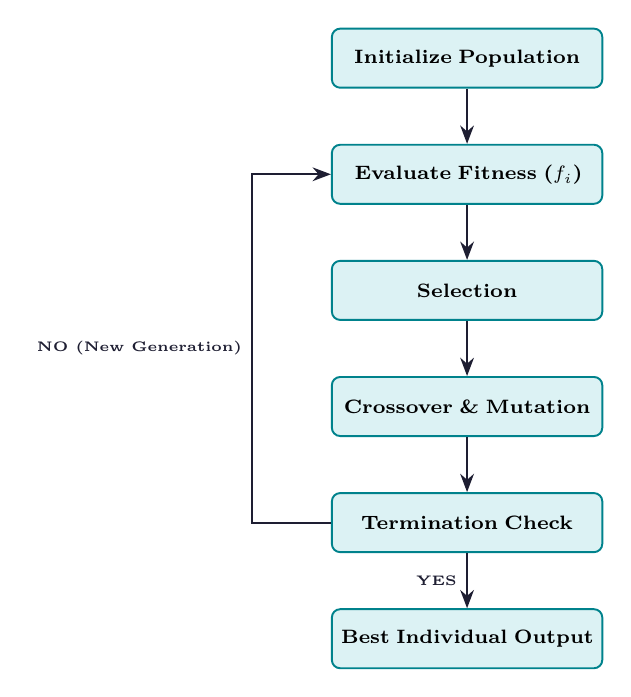
\begin{tikzpicture}[
  node distance=0.7cm and 1.5cm,
  block/.style={rectangle, draw=myteal, fill=hdrteal, text width=3.2cm, align=center, minimum height=0.75cm, font=\scriptsize\bfseries, rounded corners=3pt, line width=0.7pt},
  arrow/.style={-Stealth, thick, color=mydark}
]
  \node[block] (s1) {Initialize Population};
  \node[block, below=of s1] (s2) {Evaluate Fitness ($f_i$)};
  \node[block, below=of s2] (s3) {Selection};
  \node[block, below=of s3] (s4) {Crossover \& Mutation};
  \node[block, below=of s4] (s5) {Termination Check};
  \node[block, below=of s5] (s6) {Best Individual Output};

  \draw[arrow] (s1) -- (s2);
  \draw[arrow] (s2) -- (s3);
  \draw[arrow] (s3) -- (s4);
  \draw[arrow] (s4) -- (s5);
  \draw[arrow] (s5) -- node[left, font=\tiny\bfseries\color{mygreen}] {YES} (s6);
  
  \draw[arrow] (s5.west) -- ++(-1.0,0) |- node[pos=0.25, left, font=\tiny\bfseries\color{myred}] {NO (New Generation)} (s2.west);
\end{tikzpicture}
\end{tcolorbox}

% ===============================================================================
\section{Simulated Annealing (SA)}
% ===============================================================================

Simulated Annealing is inspired by the physical process of annealing in metallurgy, where a metal is heated to a high temperature and cooled slowly to minimize internal energy, forming a perfect crystal lattice.

\subsection{The Metropolis Acceptance Criterion}
SA allows uphill moves (accepting worse designs) to escape local minima. Let the change in objective value be $\Delta E = f(\mathbf{x}_{new}) - f(\mathbf{x}_{old})$.

\begin{tcolorbox}[formulabox, title={Metropolis Criterion Equations}]
\begin{itemize}[leftmargin=*, itemsep=3.5pt, topsep=0pt]
  \item If $\Delta E < 0$ (improvement), the new state is \textbf{always accepted}: $P(Accept) = 1$.
  \item If $\Delta E \ge 0$ (worse state), the new state is accepted with a \textbf{Boltzmann probability}:
    \begin{equation}
      P(Accept) = \exp\left( -\frac{\Delta E}{T} \right)
    \end{equation}
    Where $T$ is the virtual temperature.
\end{itemize}
\par\vspace{3pt}
As the temperature $T$ is slowly reduced using a cooling schedule (e.g., $T_{k+1} = \alpha T_k$ with $0.8 \le \alpha < 1.0$), the probability of accepting worse moves approaches 0, and the algorithm converges to the global minimum.
\end{tcolorbox}

% ===============================================================================
\section{Swarm Intelligence Algorithms}
% ===============================================================================

Swarm intelligence algorithms mimic the collective behavior of decentralized, self-organized biological swarms.

\subsection{Particle Swarm Optimization (PSO)}
PSO is inspired by bird flocking. A swarm of particles moves through the design space, where each particle tracks its own personal best position ($\mathbf{p}_{best, i}$) and the swarm's global best position ($\mathbf{g}_{best}$).

\begin{tcolorbox}[formulabox, title={PSO Particle Update Equations}]
At generation $t+1$, the velocity vector $\mathbf{v}_i$ and position vector $\mathbf{x}_i$ of particle $i$ are updated as:
\begin{equation}
  \mathbf{v}_i^{(t+1)} = w \mathbf{v}_i^{(t)} + c_1 r_1 \left( \mathbf{p}_{best, i} - \mathbf{x}_i^{(t)} \right) + c_2 r_2 \left( \mathbf{g}_{best} - \mathbf{x}_i^{(t)} \right)
\end{equation}
\begin{equation}
  \mathbf{x}_i^{(t+1)} = \mathbf{x}_i^{(t)} + \mathbf{v}_i^{(t+1)}
\end{equation}
Where:
\begin{itemize}[leftmargin=*, itemsep=2.0pt, topsep=0pt]
  \item $w$ is the \textbf{inertia weight} regulating momentum.
  \item $c_1$ (cognitive parameter) and $c_2$ (social parameter) are acceleration constants.
  \item $r_1, r_2$ are random numbers uniformly distributed in $[0, 1]$.
\end{itemize}
\end{tcolorbox}

\subsection{Swarm Variants: DE, BFA, and ACO}
\begin{itemize}[leftmargin=*, itemsep=4pt]
  \item \textbf{Differential Evolution (DE):} A vector-based evolutionary algorithm that creates new candidate vectors by adding weighted differences between random population vectors to a target vector, followed by crossover and selection.
  \item \textbf{Bacterial Foraging Algorithm (BFA):} Mimics the chemotaxis (swimming and tumbling), reproduction, and dispersal behaviors of E. coli bacteria.
  \item \textbf{Ant Colony Optimization (ACO):} Mimics the foraging behavior of real ants, which communicate path lengths using chemical pheromones.
\end{itemize}

\begin{tcolorbox}[formulabox, title={Ant Colony Pheromone Update Rule}]
The pheromone level $\tau_{ij}$ on path segment $(i, j)$ is updated after each iteration as:
\begin{equation}
  \tau_{ij} = (1 - \rho)\tau_{ij} + \sum_{k=1}^m \Delta \tau_{ij}^k
\end{equation}
Where:
\begin{itemize}[leftmargin=*, itemsep=2.0pt, topsep=0pt]
  \item $\rho$ is the \textbf{pheromone evaporation rate} ($0 < \rho \le 1$), preventing infinite accumulation.
  \item $\Delta \tau_{ij}^k$ is the pheromone deposited by ant $k$: $\Delta \tau_{ij}^k = \frac{Q}{L_k}$ if ant $k$ traversed segment $(i, j)$ (where $L_k$ is the total path length, and $Q$ is a constant).
\end{itemize}
\end{tcolorbox}

\newpage

% ===============================================================================
% MANDATORY QUICK REVISION PAGE
% ===============================================================================
\begin{center}
  {\large\bfseries\color{myred} Quick Revision --- Module 6}\\[3pt]
  {\small\color{mydark} Advanced Swarm Algorithms $|$ OE-EC704B}
\end{center}
\noindent{\color{myred}\rule{\linewidth}{1.2pt}}
\vspace{4pt}

\begin{tcolorbox}[formulabox, title={\textbf{Key Concepts \& Swarm Metrics}}]
\renewcommand{\arraystretch}{1.45}
\begin{tabularx}{\linewidth}{B{5.0cm} X}
Selection Probability & $p_i = f_i / \sum f_j$ \quad (Roulette Wheel). \\[4pt]
Boltzmann Probability & $P(Accept) = \exp(-\Delta E / T)$ \quad (Simulated Annealing). \\[4pt]
PSO Velocity Update & $\mathbf{v}_i^{(t+1)} = w \mathbf{v}_i^{(t)} + c_1 r_1 (\mathbf{p}_{best} - \mathbf{x}_i) + c_2 r_2 (\mathbf{g}_{best} - \mathbf{x}_i)$. \\[4pt]
PSO Position Update & $\mathbf{x}_i^{(t+1)} = \mathbf{x}_i^{(t)} + \mathbf{v}_i^{(t+1)}$. \\[4pt]
ACO Pheromone Update & $\tau_{ij} \leftarrow (1-\rho)\tau_{ij} + \sum \Delta \tau_{ij}^k$ \quad ($\rho$ is evaporation rate). \\
\end{tabularx}
\end{tcolorbox}

\begin{tcolorbox}[defbox, title={\textbf{One-Line Definitions}}]
\begin{itemize}[leftmargin=*, itemsep=2.5pt, topsep=0pt]
  \item \textbf{Meta-heuristic Algorithm:} A high-level search heuristic designed to find, generate, or select a search path to solve global optimization problems.
  \item \textbf{Crossover Operator:} A GA operator that recombines parts of two parent chromosomes to produce offspring.
  \item \textbf{Elitism:} A GA technique that copies the best-performing chromosomes directly to the next generation without changes.
  \item \textbf{Annealing Cooling Schedule:} A function detailing how the virtual temperature $T$ is systematically reduced during Simulated Annealing.
  \item \textbf{Inertia Weight ($w$):} A PSO parameter controlling the influence of a particle's historical velocity on its current trajectory.
  \item \textbf{Chemotaxis:} The direct movement of E. coli bacteria along chemical gradients, consisting of alternating swims and tumbles.
\end{itemize}
\end{tcolorbox}

\begin{tcolorbox}[exambox, title={\textbf{Frequently Asked / Viva Questions}}]
\begin{enumerate}[topsep=0pt, label=\textbf{Q\arabic*.}, itemsep=5pt]
  \item \Q{Explain the three primary operators used in standard Genetic Algorithms.}
    The operators are: Selection (copies high-fitness chromosomes to the mating pool), Crossover (recombines genetic sequences from parent pairs to create offspring), and Mutation (randomly alters genes to maintain population diversity).
  \item \Q{How does Roulette Wheel selection work?}
    In Roulette Wheel selection, the selection probability of an individual is proportional to its fitness value. Highly fit individuals occupy a larger slice of the virtual wheel, increasing their chances of being chosen.
  \item \Q{What is simulated annealing and what is its thermodynamic analogy?}
    SA is a global optimization algorithm. Its thermodynamic analogy is the slow cooling (annealing) of a molten metal to achieve a low-energy, highly structured crystal lattice, which corresponds to the global minimum.
  \item \Q{Why does Simulated Annealing accept worse designs, and how does it prevent divergence?}
    It accepts worse designs to climb out of local minima traps. It prevents divergence by reducing the acceptance probability ($e^{-\Delta E/T}$) as the virtual temperature $T$ cools, making the search purely local at the end.
  \item \Q{Write down the velocity update equation for Particle Swarm Optimization (PSO).}
    $\mathbf{v}_i^{(t+1)} = w \mathbf{v}_i^{(t)} + c_1 r_1 \left( \mathbf{p}_{best, i} - \mathbf{x}_i^{(t)} \right) + c_2 r_2 \left( \mathbf{g}_{best} - \mathbf{x}_i^{(t)} \right)$.
  \item \Q{Define the cognitive and social terms in the PSO update equations.}
    The cognitive term ($c_1 r_1(\mathbf{p}_{best} - \mathbf{x})$) pulls the particle toward its own personal historical best. The social term ($c_2 r_2(\mathbf{g}_{best} - \mathbf{x})$) pulls the particle toward the global best found by the entire swarm.
  \item \Q{What is the role of pheromone evaporation in Ant Colony Optimization (ACO)?}
    It systematically decreases the pheromone levels on all paths ($1-\rho$). This prevents the algorithm from getting stuck in early sub-optimal paths by allowing alternative pathways to compete.
  \item \Q{How does the Differential Evolution (DE) algorithm generate new candidate vectors?}
    It creates new trial vectors by adding a weighted difference vector between two random population members to a third vector, followed by crossover and selection.
  \item \Q{List the three operational steps of the Bacterial Foraging Algorithm (BFA).}
    Chemotaxis (swimming and tumbling), Reproduction (splitting healthy bacteria), and Elimination and Dispersal (dispersing bacteria randomly to model environmental shocks).
  \item \Q{What is Elitism in Genetic Algorithms and why is it used?}
    Elitism is the process of copying the absolute best individual(s) directly to the next generation without crossover or mutation. This prevents the loss of the best found design due to random operators.
\end{enumerate}
\end{tcolorbox}

\end{document}
